\section{Introducción}

Los vehículos VTVL son tan viejos como el primer alunizaje. Traen en si varias ventajas frente a otros vehículos voladores como la gran reducción de espacio necesario para despegar y aterrizar. Esto no es un detalle menor dado que la mayor parte de la superficie terrestre de la tierra no son pistas de aterrizaje si no más bien terreno formado naturalmente.

Este documento propone el diseño, simulación, control y fabricación de un vehículo eléctrico con capacidades VTVL que podría usarse para transporte de insumos médicos a zonas de acceso limitado o para investigar el fenómeno del \textit{fuel sloshing} en vehículos con tanques esbeltos.

\begin{figure}[htb]
    \centering
    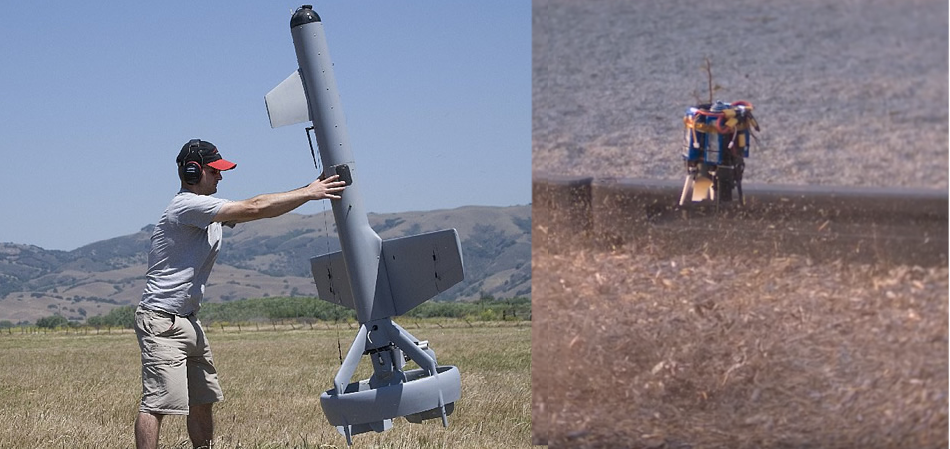
\includegraphics[width=0.8\linewidth]{fig/vbat_icarus.png}
    \caption{Dos vehículos VTVL eléctricos modernos. ``VBat'' (Izq.) y ``Ikarus'' (Der.).}
    \label{fig:vbat_icarus}
\end{figure}

Los vehículos VTVL eléctricos son propulsados por hélices en su mayoría y constan casi siempre de 3 o más propulsores en un arreglo simétrico y plano. Recientemente hay un interés por la construcción de vehículos de una sola hélice por la buena relación empuje--peso que tienen. Sin embargo, estos vehículos no vienen sin sus complicaciones: 

\begin{itemize}
    \item La rotación dada al aire por la hélice causa un momento en el eje de propulsión que es contrarrestado en vehículos multirrotores.
    \item Inclinar al rotor durante su funcionamiento causa una fuerza perpendicular a la dirección de inclinación conocido como el efecto giroscópico. 
\end{itemize}

El primer punto es mitigado fácilmente agregando álabes a la salida del chorro para enderezar el flujo y contrarrestar la rotación. El segundo punto solo se resuelve conociendo las ecuaciones de momento angular y controlando actuadores con un sistema de control a lazo cerrado. Los sistemas vistos en la figura \ref{fig:vbat_icarus} tienen la particularidad de poder ser representados con relativa facilidad usando un solo marco de referencia inercial para el cálculo de las ecuaciones de momento angular. 

\subsection{Estudio - Agua como propelente}
Se estudió también la posibilidad de propulsar el vehículo con agua a presión. La figura \ref{fig:bottlerocket} muestra los resultados de una simulación de un vehículo pequeño de aluminio con un tanque a presión lleno en parte de agua y aire a 200 bar. En el mejor de los casos se llegaba a un tiempo de vuelo cercano a los 4 segundos que no es suficiente para comprobar un sistema de control. 

Para optimizar este problema se modificaba

\begin{itemize}
    \item Diámetro de la tobera -- más empuje vs. menos tiempo de vuelo controlado
    \item Volumen de agua -- más tiempo de vuelo vs. mayor peso de vehículo
\end{itemize}


\begin{figure}[htb]
    \centering
    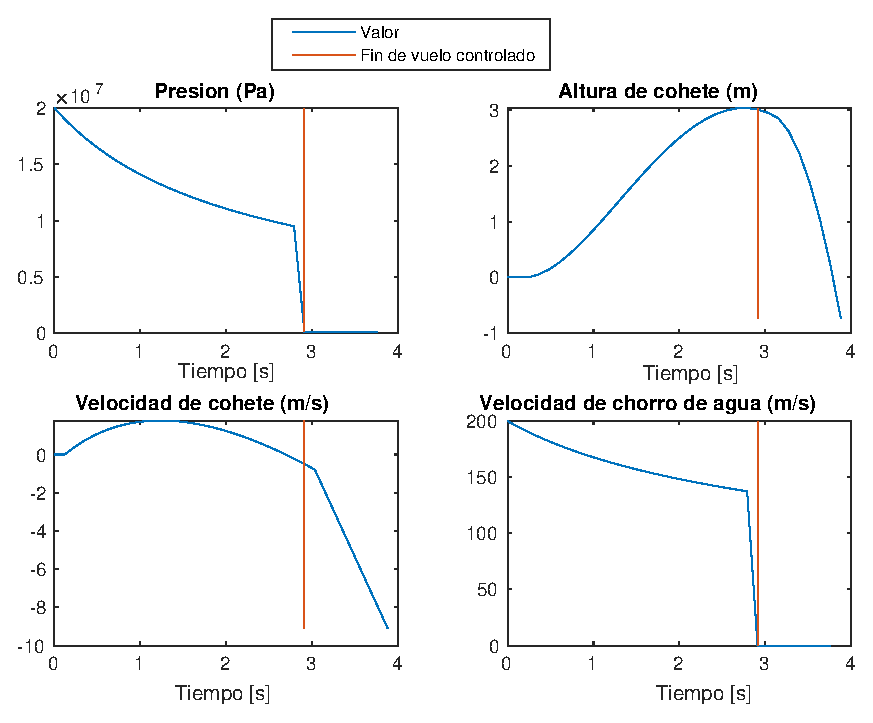
\includegraphics[width=0.8\linewidth]{fig/bottlerocket}
    \caption{Análisis preliminar para un vehículo propulsado por agua a presión. La presión es absoluta.}
    \label{fig:bottlerocket}
\end{figure}

\newpage



